\section{MGnify's rRNA-prediction subworkflow}\label{sec:Ported-version-of-MGnify}

\subsection{Detailed step-by-step analysis of the MGnify rRNA-prediction subworkflow}\label{subsec:Interpretation}
To facilitate the interpretation of the rRNA-prediction subworkflow, the CWL scripts~\cite{noauthor_pipeline-v5_2023} and CWL-Viewer tool~\cite{noauthor_common_nodate} were employed to investigate the subworkflow. Furthermore, the subworkflow was visualized (\Cref{fig:rRNA-prediction-subWF}) using the online visualization application drawio~\cite{noauthor_jgraphdrawio_nodate}.\\
A detailed step-by-step description of the subworkflow is shown in \Cref{fig:rRNA-prediction-subWF}. The workflow comprises the following steps: CMsearch conducts a similarity search using the quality-checked reads (input\textunderscore sequences) and Rfam SSU and LSU covariance models, and outputs a ranked list of top-scoring hits and hit alignments (matches). The matches of CMsearch and a clan information file, a file containing a list of clans, CL00111 (SSU) and CL00112 (LSU), are directed to cmsearch-deoverlap. Cmsearch-deoverlap removes low-score overlapping hits from the CMsearch output, which are found in the same clan and outputs deoverlapped matches. The awk based script extract\textunderscore coords\textunderscore awk extracts the target sequence name, accession number, sequence start, and sequence end from the deoverlapped matches and formats them to be suitable as an input for esl-sfetch-manyseqs. Esl-sfetch-manyseqs, a tool used to extract sequences or subsequences from an indexed sequences file~\cite{eddy_hmmer_nodate},  receives the sequences matched with their coordinates as well as the indexed sequence file in SSI format from esl-sfetch-index and outputs a FASTA file containing the sliced sequences. Get\textunderscore subunits extracts the SSU and LSU sequences and separates them into two different FASTA files. MAPseq classifies the SSU and LSU sequences, using the corresponding SILVA SSU/LSU database and SSU/LSU taxonomy file. Mapseq2biom receives the classifications from MAPseq and the corresponding SILVA SSU/LSU OTU table, and 
produces three outputs: A TSV file (otu\textunderscore tsv) containing OTU IDs, abundance, taxonomy, and NCBI taxonomy IDs. A second TSV file (otu\textunderscore tsv\textunderscore notaxid) excluding the NCBI taxonomy IDs. And a third file (otu\textunderscore txt) containing abundance and taxonomy, that serves as a Krona input. Biom convert is used to convert otu\textunderscore tsv\textunderscore notaxid to HDF5 and JSON formats. Lastly, Krona visualizes the taxa abundance table  (otu\textunderscore txt) in the form of a relative abundance pie chart.

\begin{figure}[H]
  \centering
  \subfloat{{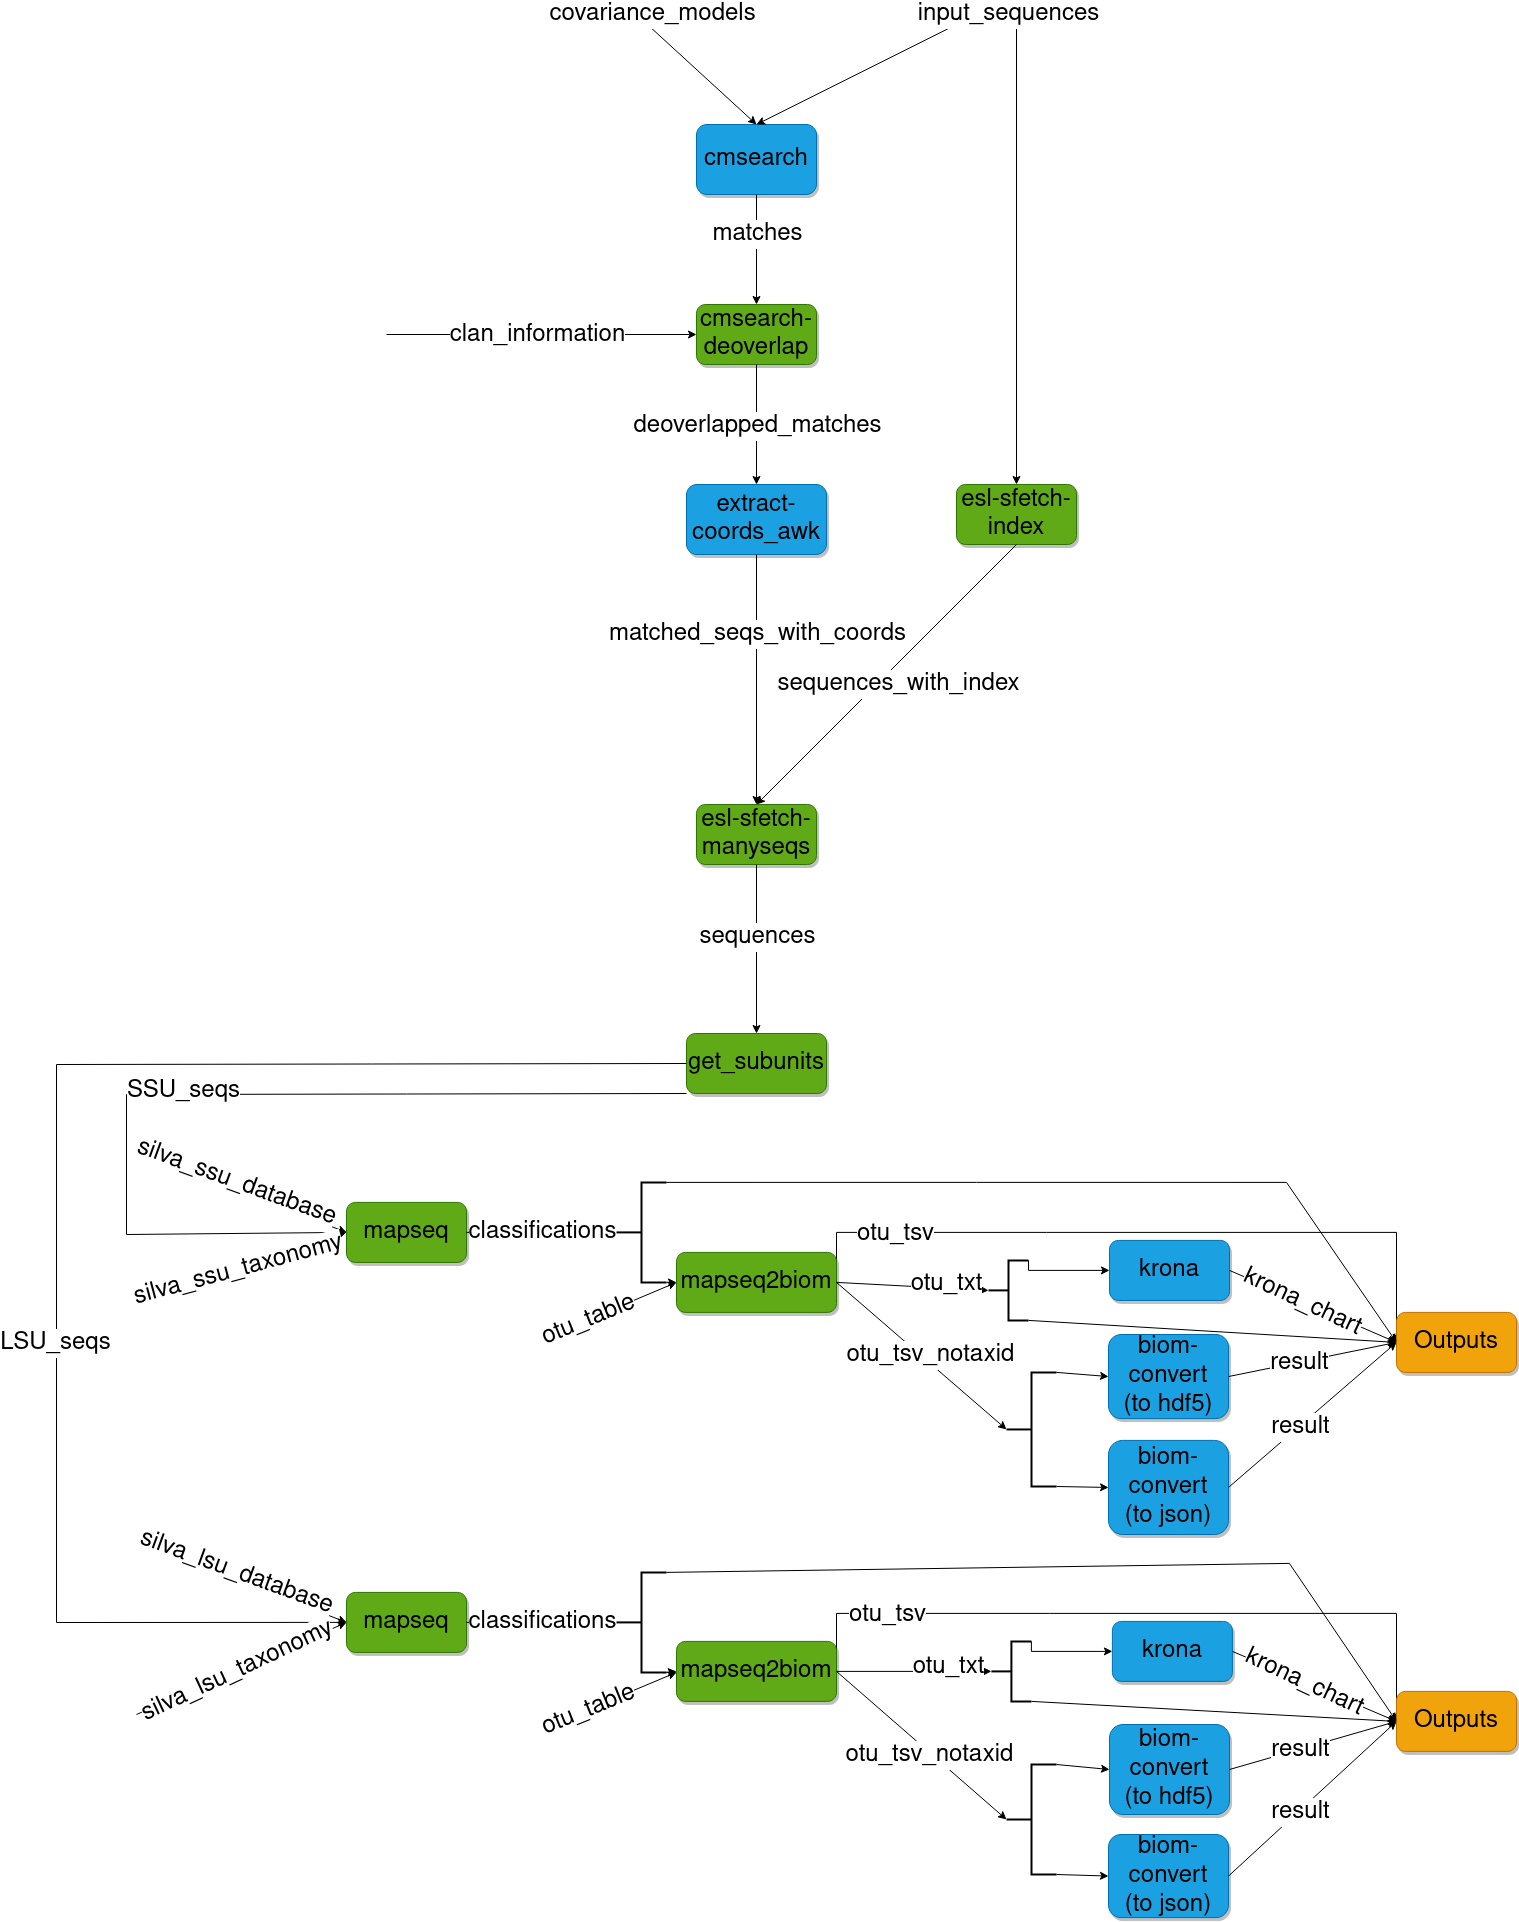
\includegraphics[scale=0.26]{figures/flowchart_rnaPredictionSubWF.drawio.png} }}%
  \captionof{figure}[MGnify's rRNA-prediction subworkflow]{\textbf{MGnify's rRNA-prediction subworkflow}. Visualized using drawio. The blue boxes show tools already existing in Galaxy. The green boxes show the tools, which were missing from Galaxy.} \label{fig:rRNA-prediction-subWF}%
\end{figure}

\subsection{Port of the rRNA-prediction subworkflow into Galaxy}\label{subsec:Ingration_to_galaxy}
Tools that were not available in Galaxy were identified. The identified tools were either replaced by existing Galaxy tools with similar functions, or a Galaxy wrapper was developed for the missing tools. Planemo, a set of command-line utilities designed to support Galaxy tool development~\cite{noauthor_welcome_nodate}, was used to test and lint the developed tool wrappers.\\
The existing wrappers for CMsearch (from the infernal package v1.1.4) had minor mistakes, which resulted in undesired Outputs~\cite{gruning_galaxy_2023}; small adjustments had to be conducted before use. CMsearch-deoverlap v0.08~\cite{nawrocki_nawrockiecmsearch_tblout_deoverlap_2023} was wrapped and integrated into Galaxy~\cite{noauthor_galaxytoolstoolsrna_toolscmsearch_deoverlap_nodate}.\\
Esl-sfetch was substituted with the functionally similar tool bedtools getfasta~\cite{noauthor_tools-iuctoolsbedtools_nodate}, which already existed as galaxy tool. In order to be able to use bedtools getfasta instead of esl-sfetch, the output created by cmsearch-deoverlap (see \Cref{fig:rRNA-prediction-subWF}) had to be formatted and converted to a regions file in BED format. The conversion was made using the Galaxy tools: Query Tabular~\cite{noauthor_tools-iuctoolsquery_tabular_nodate}, Text reformatting~\cite{noauthor_galaxytoolstoolstext_processingtext_processing_nodate}, and Concatenate two BED files~\cite{noauthor_tools-devteamtool_collectionsgopsconcat_nodate}.\\
Since the version of MAPseq~\cite{rodrigues_mapseq_2023} used by MGnify (v1.2.3), was not available on bioconda, the latest version 2.1.1 ~\cite{noauthor_mapseq_nodate} was adopted for the wrapper~\cite{noauthor_tools-iuctoolsmapseq_nodate}. Furthermore, the tool mapseq2biom~\cite{noauthor_pipeline-v5toolsrna_predictionmapseq2biommapseq2biompl_nodate} was included as an option in the MAPseq wrapper (\Cref{fig:MAPseq}).\\
The Galaxy wrapper for Krona v2.7.1~\cite{noauthor_tools-iuctoolstaxonomy_krona_chart_nodate} existed already and was adopted as-is (\Cref{fig:rRNA-prediction-subWF,fig:Galaxy_WF_part2}).\\
 Biom convert (from the biom-format package v2.1.14~\cite{noauthor_tools-iuctoolsbiom_format_nodate}) had minor mistakes, which resulted in Errors or undesired Outputs~\cite{noauthor_galaxy_2023}; small adjustments had to be conducted before use (\Cref{fig:rRNA-prediction-subWF,fig:Galaxy_WF_part2}).\\


